\section{Background}
\label{sec:Background}
In this chapter, we will discuss the backgrounds of the transformation that should be developed. We will start with JIAC (the target of the transformation), BPMN (the model that is being used), followed by VSDT (the existing modeling and transformation framework to JIAC that should be extended), and JET (the technology that will help us to implement the transformation).
\subsection{JIAC(Java-based Intelligent Agent Componentware)}
JIAC \cite{11,15,4,1} is a Java-based agent architecture and framework that was developed to simplify the development of software agents. The framework supports the entire software development process of a software agent system, from the design, implementation, and deployment of the system.The JIAC framework provides features such as FIPA compliant communication,
Believe-Desire-Intention (BDI) reasoning, strong migration, web-service
connectivity and others. Further it provides high security (Common Criteria EAL3,
certified by the Federal Office for Information Security of Germany, BSI) and advanced
accounting mechanisms, making it suitable for the use in industrial and
commercial applications. The JIAC framework comes with a runtime environment
and a toolsuite for the creation of agents. \\\\ A typical JIAC Application consists of \textit{AgentNodes}, \textit{Agents}, and \textit{AgentBeans} (see also Figure 1).
\begin{figure}[h]
	\centering
		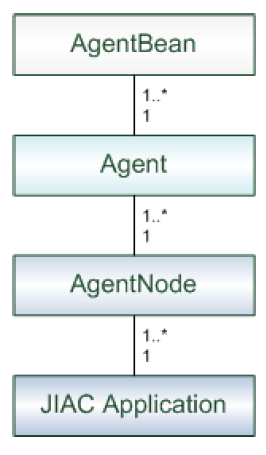
\includegraphics[width=0.25\textwidth]{images/jiac_basic.png}
		\caption{Jiac Basic concepts and their structural relationships \cite{11}}
	\label{fig:jiac_basic}
\end{figure}
An \textit{AgentNode} is a Java VM providing the runtime infrastructure for agents, such
as discovery services, white and yellow pages services, communication infrastructure. A
JIAC application consists of one or more AgentNodes. Normally, there is one AgentNode
per physical machine. The AgentNode comes ready-to-run, but can be adapted to the
needs of the target environment and can also be extended by additional components,
so-called AgentNodeBeans.\\
Each AgentNode may run several \textit{Agents}. Agents provide services to other agents
and comprise lifecycle, execution cycle and a memory. An agent can use infrastructure
services in order to find other agents, to communicate to them and to use their services.
Skills and abilities of the agent can be extended by so-called AgentBeans.\\
\textit{AgentBeans} is the mean to implement the functionality. They are plugged into agents
and provide services (so-called Actions) to other agents. AgentBeans have a lifecycle.

\subsection{BPMN(Business Process Modelling Notation)}
BPMN \cite{6} is a standard Notation for modelling business processes, initially published by the BPMI which is later adopted by the OMG(Object Management Group). A business process diagramm (as seen in Figure 2) can be compared to UML's activity diagram.
\begin{figure}[h]
	\centering
		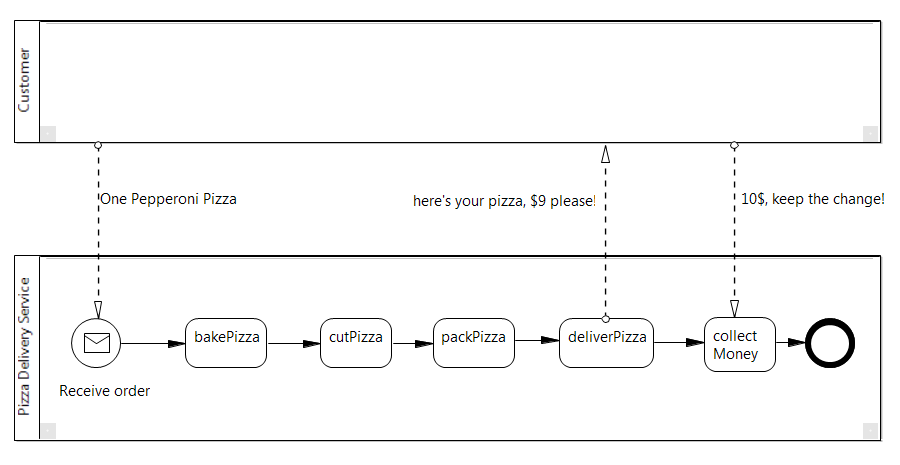
\includegraphics[width=0.90\textwidth]{images/bpmn_sampl.png}
	\caption{A simple Business Process Diagramm}
	\label{fig:bpmn_sampl}
\end{figure}\\
BPMN was made to provide a notation that is understandable by all business users, creating a brige for the gap between the business process design and the process implementation. With the mapping of BPMN to Agents, we hope to be able to increase the spreading of the multi agent systems in the business world.

To provide a rough overview on how Agent technology can support the implementation of Business Processes let us take a look on this mapping example of BPMN elements to Agents. A Pool in a Business Process Diagram can represent an Agent, which are able to communicate with other agents (another pool) through messages (represented with the BPMN MessageFlows). Agents can react to Events. To fully implement the transformation a detailed mapping is needed and will be developed in the scope of this work. 

\subsection{VSDT(Visual Service Design Tool)}
The VSDT \cite{5,2,3,1} is a well-equipped BPMN editor that is independent of any specific target language. Thus, while the usual transformation to BPEL, as well as other transformations, is included, the VSDT can easily be extended with additional export functionality targeting other languages. It was developed in early 2007 as a Diploma Thesis at the TU Berlin and since then it has been continuously extended. Since it's initial development, VSDT's transformation framework is designed to be extensible and reuseable. This allows the development of a new transformation to be easier. For this purpose the transformation process is subdivided into several stages: 
\begin{enumerate}
	\item \textit{Validation}: Validate the input model.
	\item \textit{Normalisation}: Prepare the input model for transformation.
	\item \textit{Structure Mapping}: Convert the input model to a block-like structure.
	\item \textit{Element Mapping}: Perform the actual mapping, create target model.
	\item \textit{Clean Up}: Remove redundancies, improve readability, etc.
\end{enumerate}

The Validation and Normalisation and Structure Mapping are mostly independent from the target language. In most cases the standard mapping provided for these stages are reuseable, which makes it possible to implement a new transformation by specifying the element mapping only. Figure 3 shows the UML Class Diagram of the transformation famework with the example transformation to BPEL.
\begin{figure}[h]
	\centering
		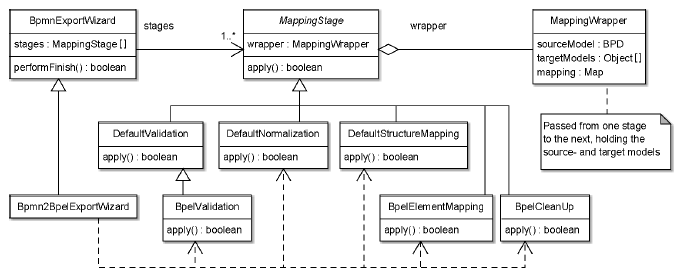
\includegraphics[width=0.90\textwidth]{images/transformation.png}
	\caption{Essential classes of the transformation framework, including the BPEL case.\cite{3}}
	\label{fig:transform}
\end{figure}\\


\subsection{JET(Java Emitter Templates)}
\textit{JET}\cite{13} is a code generating framework, developed as a part of the Eclipse Modelling Project \cite{14}. JET uses templates to transform the model into any kinds of code artifacts such as java, html, xml or even plain text. \\\\
\textit{JET templates} uses a JSP-like syntax which makes it easy to write and understand. A set of JET templates is called transformation. It is possible to build this transformation with a main template which acts as a visitor and runs through the model, and this main template will then use other templates which handle a specific element of the model. For example, in UML to Java transformation you can have special templates that handles the package, class, variables and methods.
